\section{Approach}

\subsection{Overview}

\begin{figure}[htbp]
\centerline{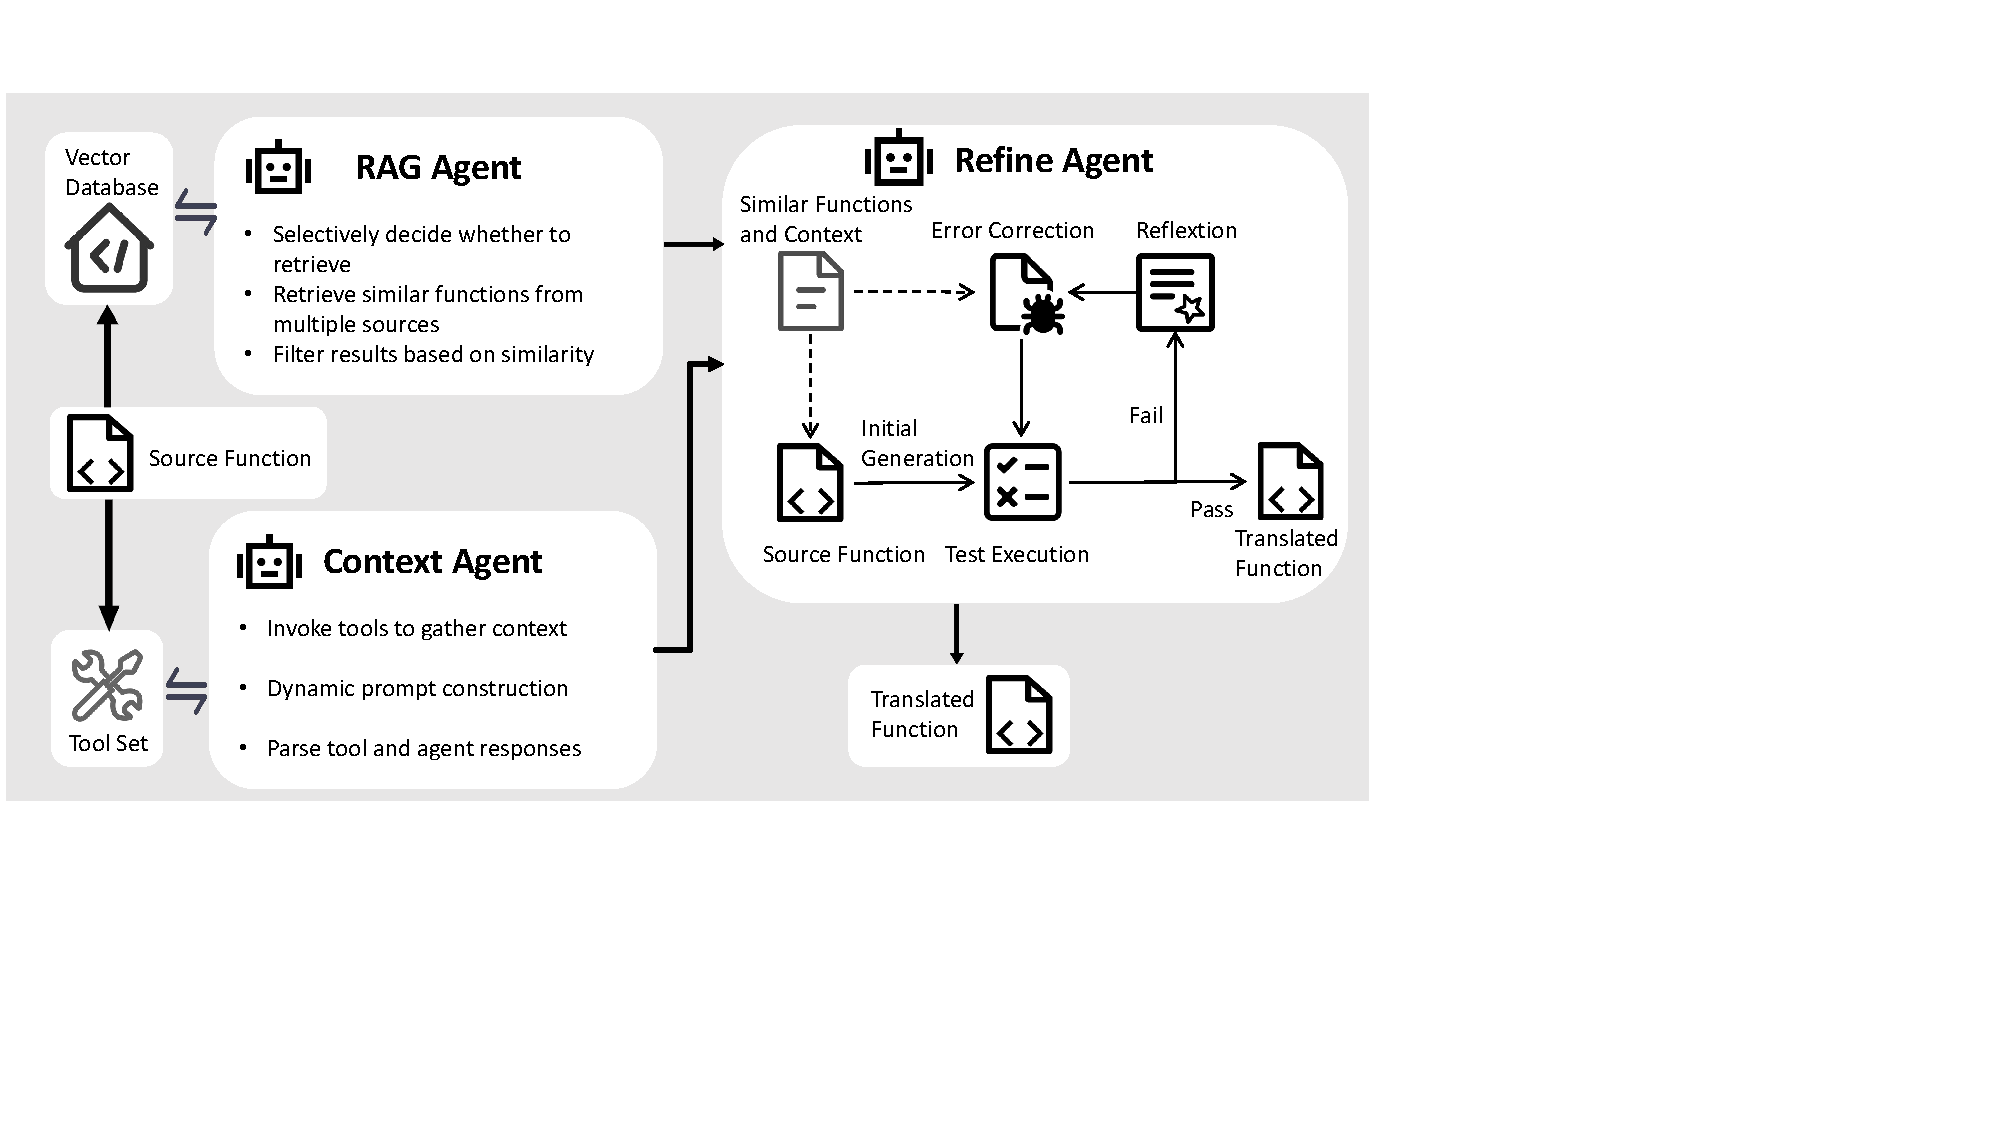
\includegraphics[width=1\linewidth]{figs/Agent.pdf}}
\caption{Overview of \toolname}
\label{fig:overview}
\end{figure}

    Fig.~\ref{fig:overview} provides an overview of the \toolname approach, which consists of three specialized agents: RAG Agent, Context Agent, and Refine Agent. During repository-aware code translation, these three agents work collaboratively to generate the final translated code. The RAG Agent is responsible for retrieving functions similar to the target function to assist in translating the source function. The Context Agent retrieves the contextual information required for translating the source function. The Refine Agent performs iterative refinement by translating the code, generating reflections based on test case execution results, and re-retrieving context according to the error information. It then uses the reflection, error messages, and updated context to fix the mistakes made in the previous iteration.

\subsection{RAG Agent}
This section details how we employ the RAG Agent to retrieve functions semantically similar to the target function to assist in translating the source function. The RAG Agent comprises four main components: Preprocessing, Selective Retrieval, Multi-Route Retrieval, and Result Filtering.

\subsubsection{Preprocessing}
To enable effective retrieval, we first store the project's metadata in a vector database. Given the metadata of a project repository, we begin by preprocessing it and generating embeddings for two distinct components of the metadata, which are subsequently stored in the vector database. The first component consists of the method bodies of all source-target translation pairs, and the second component includes the function names of all methods in the target repository. These two components are stored separately in two vector databases, referred to as the pair store and the name store, respectively.

\subsubsection{Selective Retrieval}
In real-world code repositories, many functions are standalone, meaning they do not reference external classes or functions. For such functions, it is unnecessary to employ the RAG process to retrieve additional information during translation. Bypassing the RAG process in these cases can conserve computational resources and prevent redundant information from adversely affecting translation quality. Therefore, before initiating the RAG process, we first enable the agent to determine whether the target function requires RAG assistance. This decision is based primarily on whether the target function is standalone and whether it exhibits sufficient simplicity. If the agent determines that RAG is not needed, the RAG process is bypassed.

\subsubsection{Multi-Route Retrieval}
If the agent determines that a target function requires the RAG process, a multi-route retrieval procedure is initiated. This procedure consists of two complementary components. The first component involves retrieving source-target translation pairs where the source function is similar to the current source function from the pair store. A hybrid retrieval strategy is employ: both dense retrieval (based on cosine similarity) and sparse retrieval (based on BM25) are utilized to independently retrieve the top-k most similar results from the pair store. These results are subsequently ranked using the Reciprocal Rank Fusion (RRF) method to produce the final top-k most relevant results. The second component involves retrieving functions from the name store based on the target function's name. Using sparse retrieval (BM25), the top-k functions with the most similar names are retrieved. If a function name exactly matches the target function name, its similarity score is set to 1.0. Finally, the results from both retrieval paths are merged to form the output of the multi-route retrieval step.

\subsubsection{Result Filtering}
Not every function retrieved through the multi-route retrieval process is beneficial for translating the source function into the target function. Including irrelevant functions as additional context can be not only unhelpful but potentially detrimental to translation quality. Therefore, it is essential to filter the retrieved results to retain only those functions that are genuinely useful.

We leverage the agent to perform this filtering operation. For each candidate function in the retrieved set, the agent compares it with the target function, considering factors such as functional similarity, structural resemblance, and referenced context. Based on this comparative analysis, the agent determines whether the candidate function is sufficiently similar to the target function to provide useful guidance for translating the source function. Functions deemed relevant are retained, while others are discarded.

\subsection{Context Agent}
This section presents how we employ the Context Agent to obtain the necessary context for repository-aware code translation. It comprises three components: Workflow, Tool Introduction, and Dynamic Prompt Construction.

\subsubsection{Workflow}
In the workflow of the Context Agent, we first construct a dynamic prompt using relevant information from the source and target functions, and use this prompt to query the agent, instructing it to decide which tool to invoke. The agent's response strictly adheres to a JSON format and includes three parameters: id (the identifier for the tool invocation), name (the name of the tool to be utilized), and args (the arguments for the tool).

After obtaining the tool invocation command from the agent, the Context Agent proceeds to call the specified tool and retrieves the corresponding output. This output is added to the context collection, and we also log relevant information from the tool invocation. We then use this information from the previous round to reconstruct a dynamic prompt and prompt the agent to continue invoking tools. This process is repeated iteratively until either the maximum number of iterations is reached or the agent determines that sufficient context has been gathered. Finally, the context collection is returned as the context retrieved by the Context Agent.

\subsubsection{Tool Introduction}
Our approach introduces five tool functions designed to help the Context Agent acquire context most pertinent to the source function's translation. In the Context Agent's workflow, the agent autonomously decides which tools to invoke based on function information and historical interaction data, and utilizes the outputs of these tools as contextual information. The following is an introduction to each of these tools:

\paragraph{get\_source\_class\_info} 

get\_source\_class\_info returns all field definitions and method signatures within the class that contains the source function. This tool helps the agent deduce the class to which an instance belongs by combining information about class instances and fields from the source function. This facilitates the agent in exploring how classes referenced in the source function are implemented in the target repository.    

\paragraph{get\_target\_class\_info}

get\_target\_class\_info retrieves all field definitions and method signatures within the class that contains the target function. Since the target function is likely to reference these predefined fields and implemented methods, this tool helps the agent understand which fields or methods may be invoked within the target function.

\paragraph{find\_target\_imports} 

find\_target\_imports retrieves all the imported classes in the file that contains the target function. These imported classes may be referenced within the target function and also reveal the dependencies of the target class.

\paragraph{find\_target\_class\_info} 

Given a class name to be searched, find\_target\_class\_info searches all field definition information and method signature information of the class matching the class name in the target repository. If the agent believes that a certain class has a high probability of being referenced in the target function, this tool function can effectively help the agent find relevant information about the class. The agent can infer which classes may be imported in the target function based on the class name, or determine if the return value and parameters of the target function signature contain external classes. Additionally, if an instance of an external class is utilized in the source function, there is a high probability that the target function will also use an instance of that class. The agent uses get\_source\_class\_info to obtain the name of the class to which the instance belongs, and then uses find\_target\_class\_info to query the implementation of the class in the target repository. This approach addresses cases where the context of the class in the source repository and the target repository is inconsistent.

\paragraph{find\_target\_method\_body} 

Given a method name and its owning class name, the find\_target\_method\_body tool function searches in the target repository for the class that matches the class name, and then looks in that class for the complete contents of the method that matches the method name, including its method signature and method body. If a method is likely to be utilized in the target function, then understanding the specific logic and functionality of the method can help the agent better utilize the method. At the same time, knowing the specific function of a method allows the agent to decide whether to use the method in the target function.

In the workflow of the Context Agent, we first require the agent to prioritize the invocation of three tool functions: get\_source\_class\_info, get\_target\_class\_info, and find\_target\_imports, in order to collect fundamental information relevant to the translation of the source function. After obtaining this basic information, the agent gains a preliminary understanding of the context required for translating the source function. Subsequently, the agent can invoke the find\_target\_class\_info and find\_target\_method\_body tool functions multiple times to gather more specific information, continuing until it determines that a sufficient amount of context has been collected for the code translation. All context retrieved through these tool calls is finally consolidated into a JSON format and provided to the Refine Agent.

\subsubsection{Dynamic Prompt Construction}
To enable the agent to accurately invoke the necessary tools, we design a dynamic prompt to query the agent. This prompt is composed of a series of static and dynamic components. Fig.~\ref{fig:dynamic_prompt} illustrates the construction process of our dynamic prompt.

\begin{figure}[htbp]
\centerline{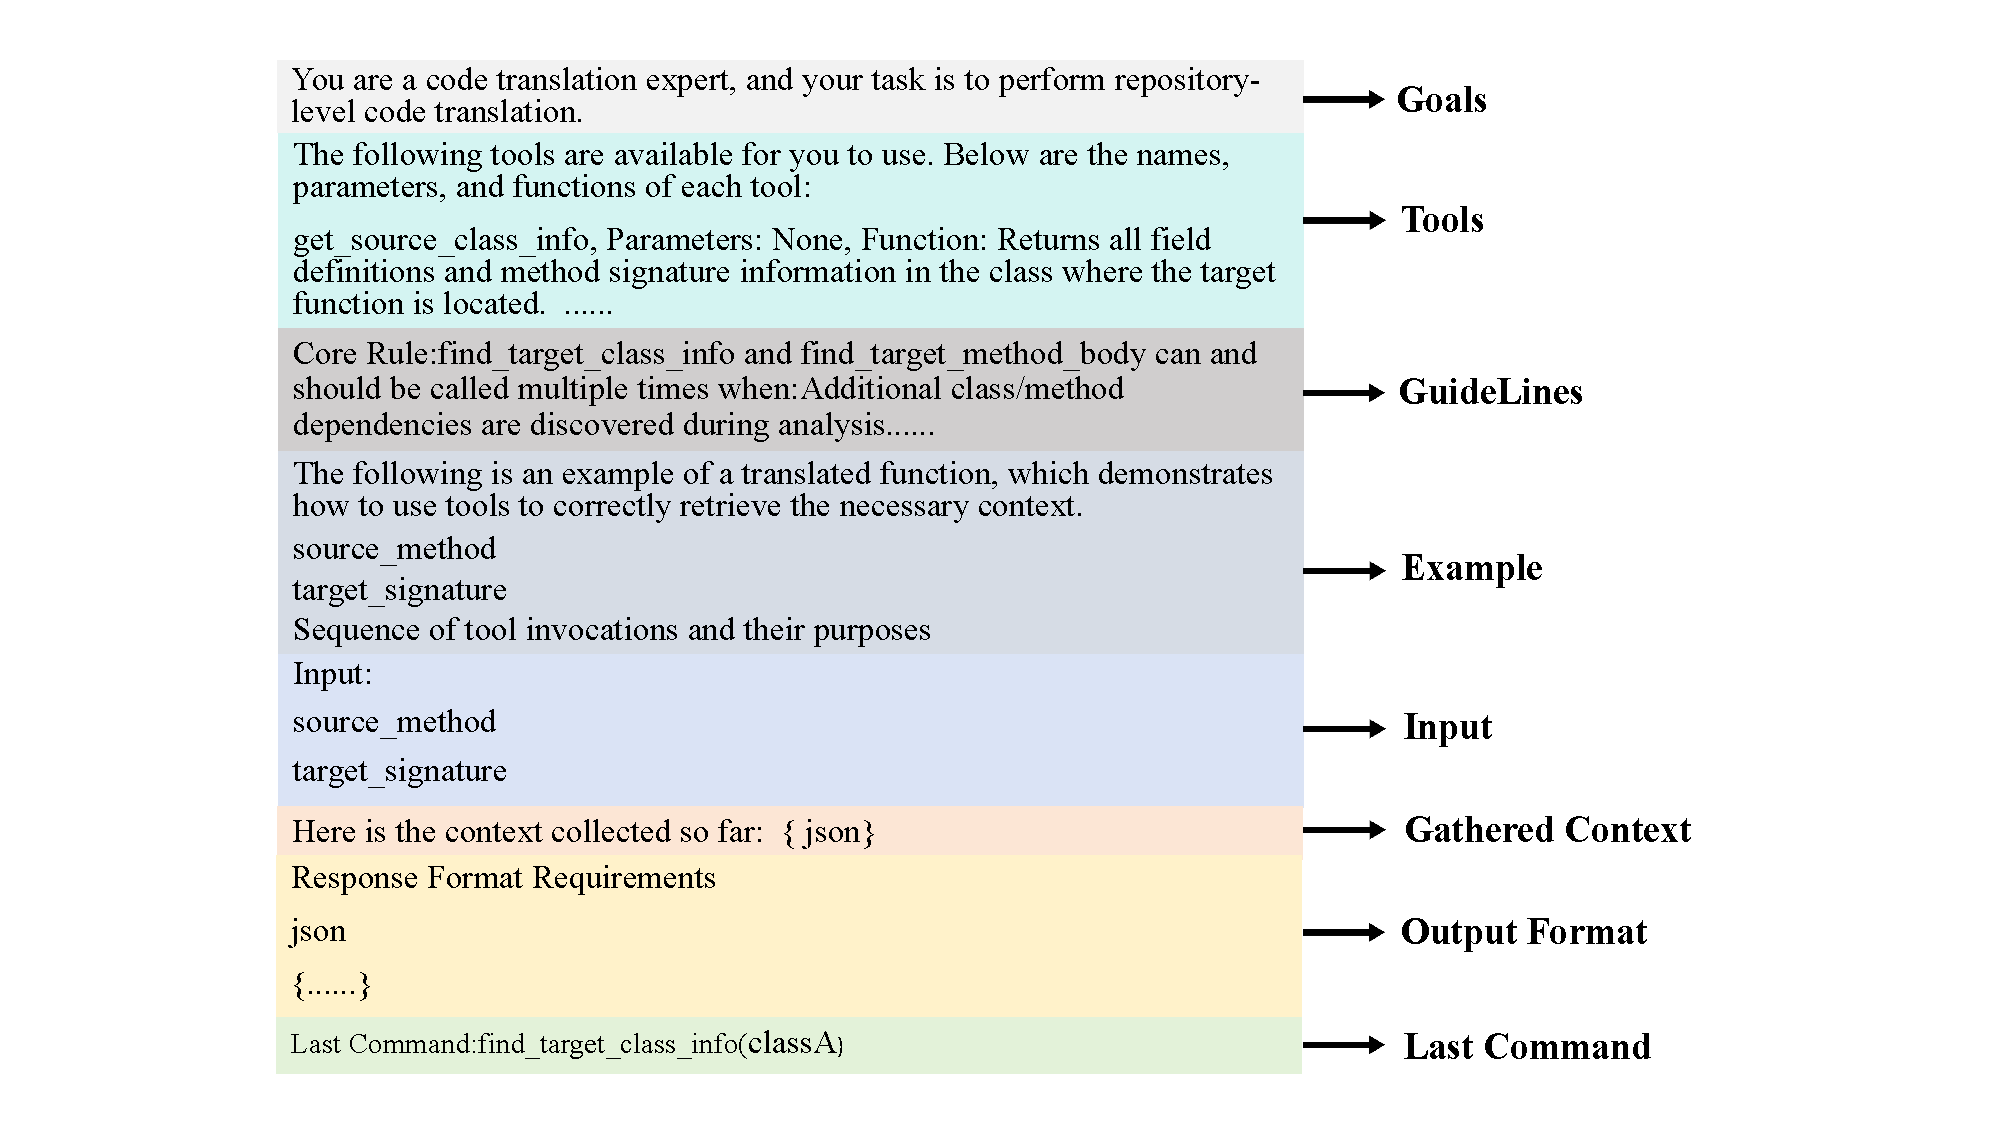
\includegraphics[width=1\linewidth]{figs/dynamic_prompt.pdf}}
\caption{An example of the dynamic prompt construction process}
\label{fig:dynamic_prompt}
\end{figure}

\paragraph{Goals (Static)} This section defines the agent's area of expertise as repository-aware code translation. It clarifies that the agent's objective is to collect the most relevant context to assist in performing repository-aware code translation.

\paragraph{Tools (Static)} In this section, we introduce all available tools, including their names, parameters, and descriptions. This serves as a reference for the agent, providing the basic information needed to correctly invoke and utilize each tool.

\paragraph{Guidelines (Static)} We provide a set of guidelines to clarify the fundamental principles for using the tools. First, the agent is instructed to prioritize calling the three tools: get\_source\_class\_info, get\_target\_class\_info, and find\_target\_imports, in order to obtain basic information relevant to translating the source function. Then, we demonstrate how to use the find\_target\_class\_info and find\_target\_method\_body tools. The agent is expected to repeatedly use find\_target\_class\_info and find\_target\_method\_body to gather sufficient context, including identifying new type dependencies, verifying interface implementations, and resolving mappings from packages to namespaces. Additionally, the agent is reminded to pay close attention to language-specific differences.

\paragraph{Example (Static)} We provide an example that includes the signatures of a source function and its corresponding target function to demonstrate how to properly use the tools to collect the necessary context for translating the source function. This example outlines each step of tool usage along with the rationale behind it, showing the agent how to progressively and effectively gather sufficient context.

\paragraph{Input (Dynamic)} This section includes the source function to be translated and the signature of the target function. It serves as the foundation for the agent to gather context, guiding the agent to collect context specifically related to the source function.

\paragraph{Gathered Context (Dynamic)} In this section, we list all the contextual information previously collected through tool invocations by the agent (this component is omitted during the first query to the agent). It acts as the agent's memory, allowing it to determine the next appropriate tool to call based on the already gathered context, enabling a step-by-step refinement to retrieve more relevant information.

\paragraph{Output Format (Static)} This section specifies the required response format for the agent, mandating that all responses strictly follow the JSON format and include three fields: id, name, and args. We explicitly instruct the agent not to include any content outside of the JSON object, such as additional text or code, and provide an example to illustrate the correct response format.

\paragraph{Last Command (Dynamic)} This section records the tool invoked in the agent's previous action along with its returned output. It serves to remind the agent to reflect on whether its current strategy may be flawed and to avoid redundant tool invocations.

\subsection{Refine Agent}
The Refine Agent serves as the core component responsible for code translation and iterative error correction through a systematic refinement process. It leverages test case execution feedback and self-reflection mechanisms to progressively enhance translation quality. The Refine Agent operates through four sequential phases: Initial Generation, Test Execution, Reflection, and Error Correction.

\subsubsection{Initial Generation}
In the initial generation phase, the Refine Agent is configure with specialized expertise in repository-aware code translation. The agent receives the source function body and target function signature as primary inputs, supplemented by contextual information from the Context Agent and similar functions from the RAG Agent.

The agent is instructed to leverage this comprehensive contextual information to produce accurate translations that account for repository-specific differences. We provide detailed guidelines and concrete examples demonstrating how to effectively utilize the additional information to resolve discrepancies between source and target repositories. The agent outputs the translated code in markdown format to ensure consistent extraction and processing.

\subsubsection{Test Execution}
Following code generation, the translated function undergoes validation through the target repository's test suite. If all test cases pass successfully, the translation is deemed complete and the process terminates. Otherwise, we systematically collect and analyze test execution results following established methodologies from existing approaches.

We categorize execution failures into four distinct types: compilation errors, test failures, runtime errors, and non-terminating executions. For each error category, we extract comprehensive diagnostic information including error logs, error classifications, output messages, and precise error locations to facilitate targeted error correction in subsequent iterations.

\subsubsection{Reflection}
The reflection phase implements a self-analysis mechanism where the agent examines the relationship between the source function, target function signature, the generated erroneous code, and the corresponding test execution results. Through this systematic analysis, the agent identifies the root causes of translation failures and formulates specific correction strategies.

This reflective process enables the agent to understand not only what went wrong but also why the error occurred, leading to more informed and targeted corrections in the subsequent iteration.

\subsubsection{Error Correction}
During the error correction phase, the agent generates an improved version of the translated code by incorporating insights from the previous iteration's code, test execution results, and reflection analysis. The prompt structure mirrors that of the initial generation phase but is enhanced with three critical components: the erroneous code from the previous iteration, detailed test execution results, and the agent's reflection and correction strategy.

The corrected code undergoes immediate re-evaluation through the test suite, initiating a new cycle of Test Execution and Reflection if errors persist. This iterative process continues until either all test cases pass successfully or the predefined maximum iteration limit is reached, ensuring both translation quality and computational efficiency.




